\section{Operationsverstärker}
Das Grundsätziche Vorgehen um Opamp-Schaltungen zu analysieren:
\begin{center}
	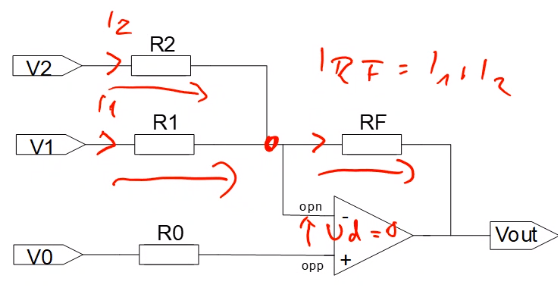
\includegraphics[width=0.5\linewidth]{Images/opamp_todo}
\end{center}

\begin{enumerate}[nosep]
	\item Verstärker, wenn Feedback auf Negativen Eingang, sonst Komperator resp. Schmitt Trigger
	\item Bestimmung $V_{opp}$
	\item $V_{opn}$ wird von Opamp auf $V_{opp}$ geregelt
	\item Eingangsströme der Eingangs-Impedanz zu opn berechnen $I_x = \frac{V_x - V_{opn}}{R_x}$
	\item Eingangsströme bei opn summieren = Strom in Feedback-Impedanz $R_F$
	\item Spannung $V_{RF}$ berechnen
	\item $V_{out} = V_{opn} - V_{RF}$
	\item Kontrollieren, ob $V_{out}$ innerhalb der Versorgung liegt.
\end{enumerate}

\subsection{Schaltungen}
\subsubsection{Buffer}
Ein Buffer hat keine Belastung an $V_{in}$ und keine Rückwirkung auf Eingang.\\
\begin{minipage}{0.25\textwidth}
	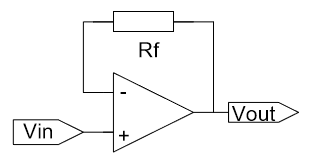
\includegraphics[width=\linewidth,keepaspectratio=true]{./Images/opamp_buffer}
\end{minipage}%%% to prevent a space
\begin{minipage}{0.25\textwidth}
	\begin{align*}
		A = 1\\
		V_{out} &= \frac{A}{1 + A}\cdot V_{in}
	\end{align*}
\end{minipage}

\subsubsection{Nicht-Invertierender Verstärker}
\begin{minipage}{0.25\textwidth}
	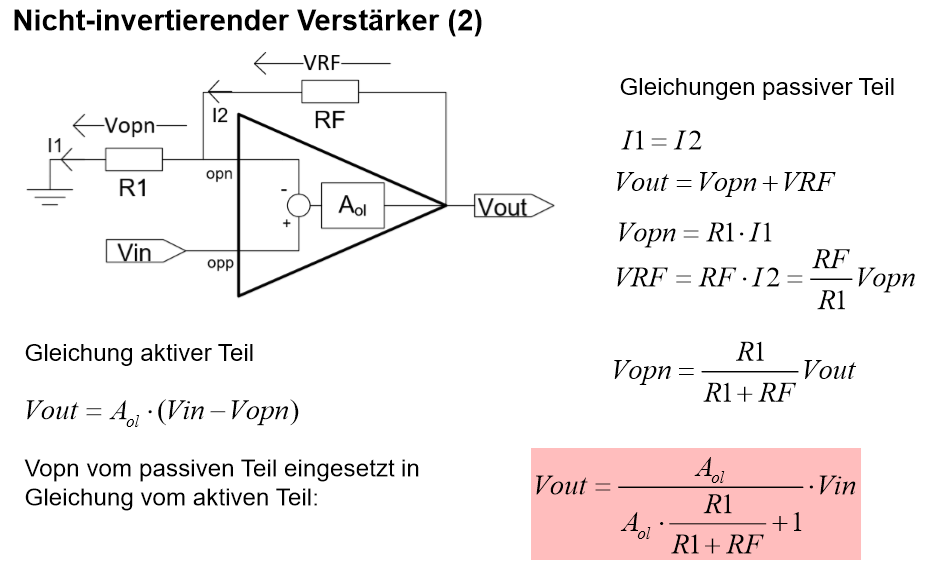
\includegraphics[width=\linewidth,keepaspectratio=true]{./Images/opamp_negatives_feedback}
\end{minipage}%%% to prevent a space
\begin{minipage}{0.25\textwidth}
	\begin{align*}
		A &= \frac{V_{out}}{V_{in}} = 1 + \frac{RF}{R1} \\
		V_{out} &= \frac{A}{A \cdot \frac{R1 + RF}{R1} + 1} \cdot V_{in}
	\end{align*}
\end{minipage}

Weil $I1 = I2$ gilt, und wenn $\frac{1}{A_{ol}} << \frac{R_1}{R_1 + R_F}$, dann gilt auch:
\[ V_{out} \approxeq \frac{R1 + RF}{R1} \cdot (V_{in} + \overbrace{V_{OS}}^{= 0})\]


\subsubsection{Invertierender Verstärker}
\begin{minipage}{0.25\textwidth}
	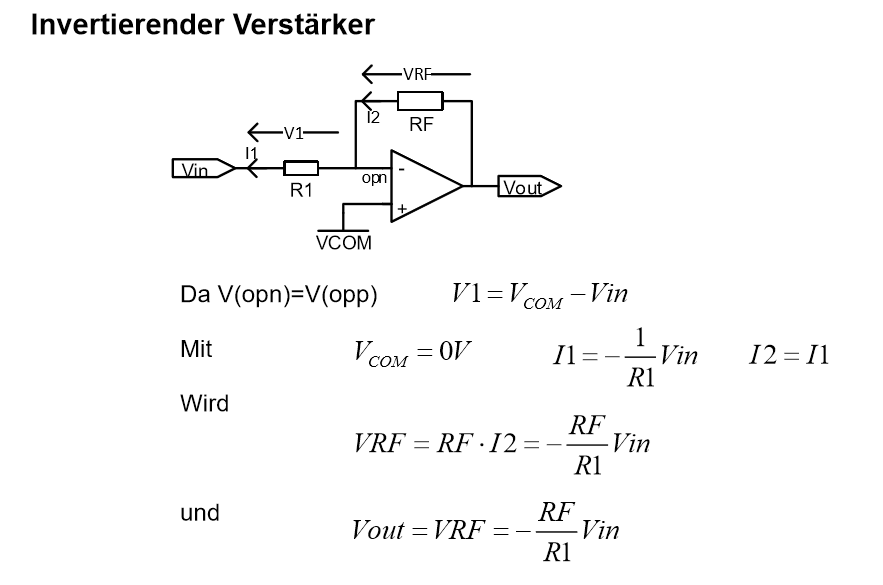
\includegraphics[width=\linewidth,keepaspectratio=true]{./Images/opamp_invertierendpng}
\end{minipage}%%% to prevent a space
\begin{minipage}{0.25\textwidth}
	\begin{align*}
		A &= \frac{V_{out}}{V_{in}} = -\frac{RF}{R1} \\
		V_{out} &= -\frac{RF}{R1} \cdot V_{in} = V_{RF}
	\end{align*}
\end{minipage}
Für nicht ideale Verstärker mit Offsetspannung:
\[
	V_{out} \approxeq \frac{R1 + RF}{R1}(V_{COM} + V_{OS}) - \frac{RF}{R1} \cdot V_{in}
\]


\subsubsection{Inventierender Addierer}
\begin{minipage}{0.20\textwidth}
	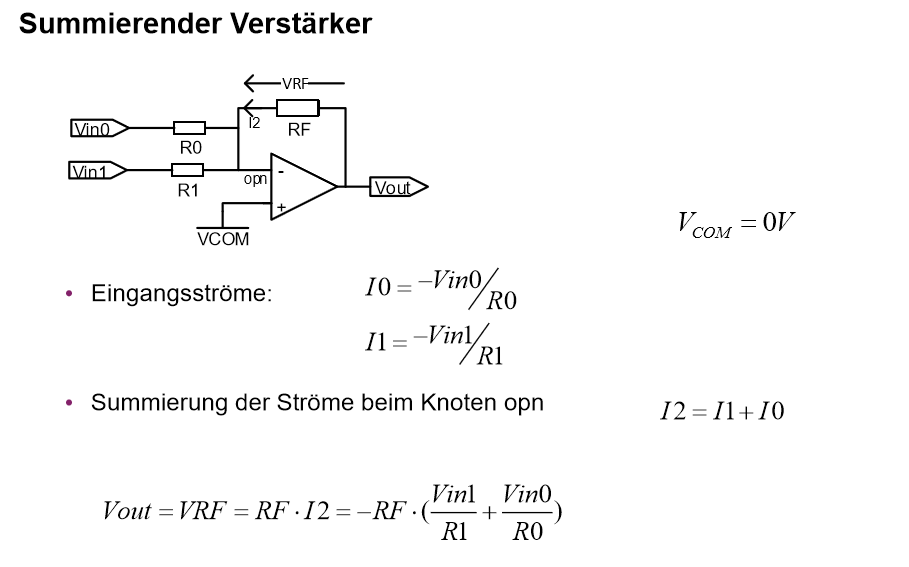
\includegraphics[width=\linewidth,keepaspectratio=true]{./Images/opamp_summierend}
\end{minipage}%%% to prevent a space
\begin{minipage}{0.30\textwidth}
	\begin{align*}
		V_{out} &= -\frac{RF}{R0} \cdot V_{in1} -\frac{RF}{R1} \cdot V_{in2} - \dots
	\end{align*}
\end{minipage}

\subsubsection{Invertierender Subtrahierer}
Mittels Superposition von $V_{in1}$ und $V_{in2}$ und Spannungsteilern kann folgende Formel gefunden werden.\\
\begin{minipage}{0.20\textwidth}
	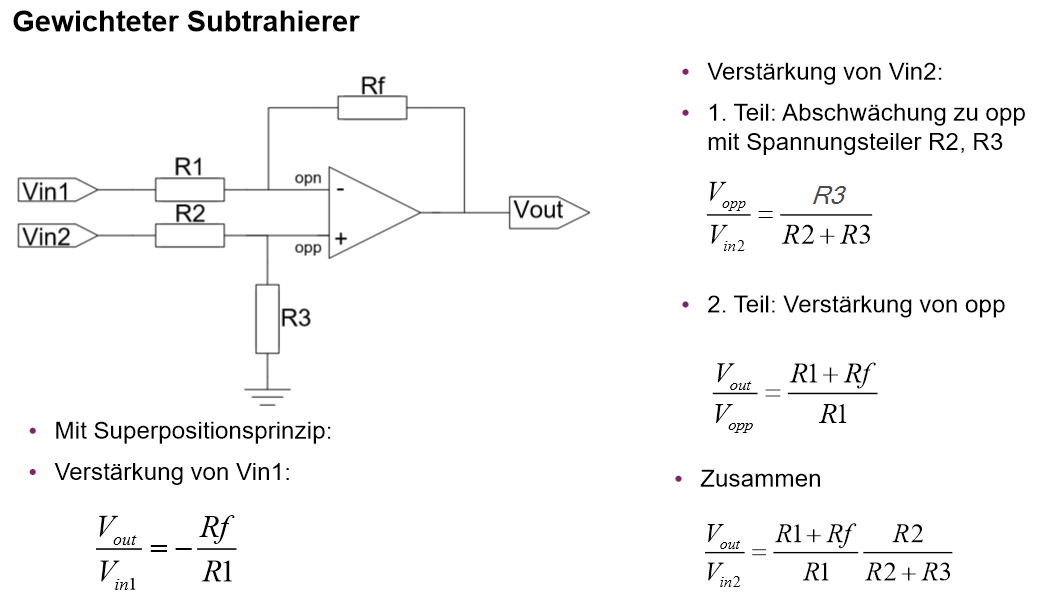
\includegraphics[width=\linewidth,keepaspectratio=true]{./Images/opamp_invertierend_subtrahierer}
\end{minipage}%%% to prevent a space
\begin{minipage}{0.30\textwidth}
	\begin{align*}
		V_{out} &= \overbrace{-\frac{Rf}{R1}}^{\frac{V_{out}}{V_{in1}}}\cdot V_{in1} \\ &+ \underbrace{\frac{R1 + Rf}{R1}}_{= \frac{V_{out}}{V_{opp}}} \cdot \underbrace{\frac{R2}{R2 + R3}}_{\frac{V_{in2}}{V_{opp}}} \cdot V_{in2}
	\end{align*}
\end{minipage}

\subsubsection{Differenzverstärker}
\begin{minipage}{0.20\textwidth}
	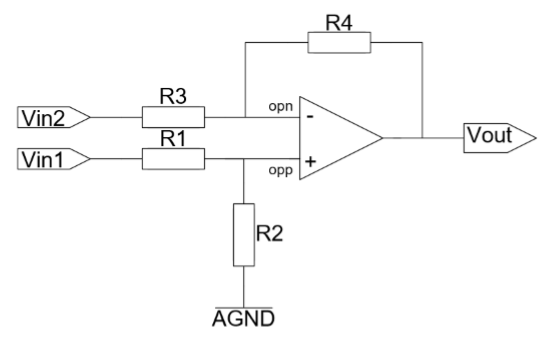
\includegraphics[width=\linewidth,keepaspectratio=true]{./Images/opamp_differenz}
\end{minipage}%%% to prevent a space
\begin{minipage}{0.30\textwidth}
	\begin{align*}
		V_{out} &= \frac{R3 +  R4}{R3} \\ &\cdot \left(\frac{R1}{R1 + R2}V_{AGND} + \frac{R2}{R1 + R2}V_{in1}\right) \\ &- \frac{R4}{R3}V_{in2}
	\end{align*}
\end{minipage}

Falls $R1=R3, R2=R4$: \[ V_{out} = V_{AGND}+ \frac{R4}{R3}(V_{in1} - V_{in2}) \]
 
\subsubsection{Mehrstuffiger Verstärker}
Verstärker können Multipliziert werden. \\
~\\\textbf{Beispiel }mit Verstärkungsfaktor \textcolor{red}{-600} wenn $V_{in}$ gegenüber GND. ACHTUNG, falls $V_{in}$ gegenüber AGND \textcolor{blue}{-601}:\\
\begin{center}
	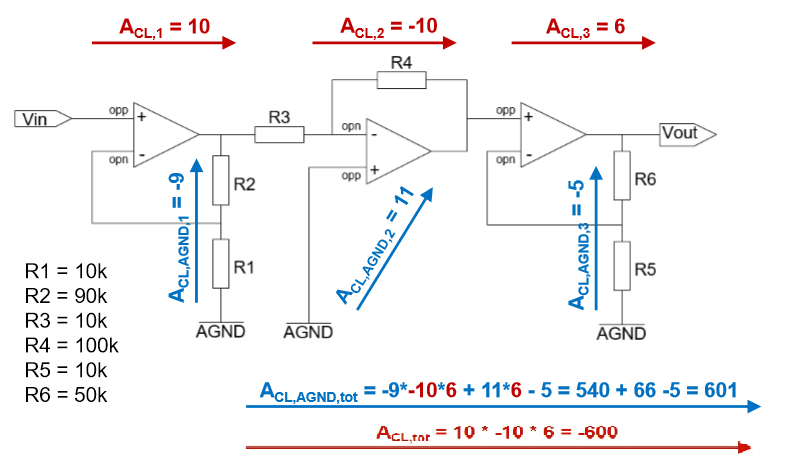
\includegraphics[width=0.8\linewidth]{Images/opamp_mehrstufig}
\end{center}
\[
V_{out} = -600\cdot V_{in} + 601\cdot V_{AGND} = -600(V_{in} - V_{AGND}) + V_{AGND}
\]

\subsubsection{T-Glied}
Hohe Verstärkung bei nicht so hohen Werteunterschieden möglich\\
\begin{minipage}{0.20\textwidth}
	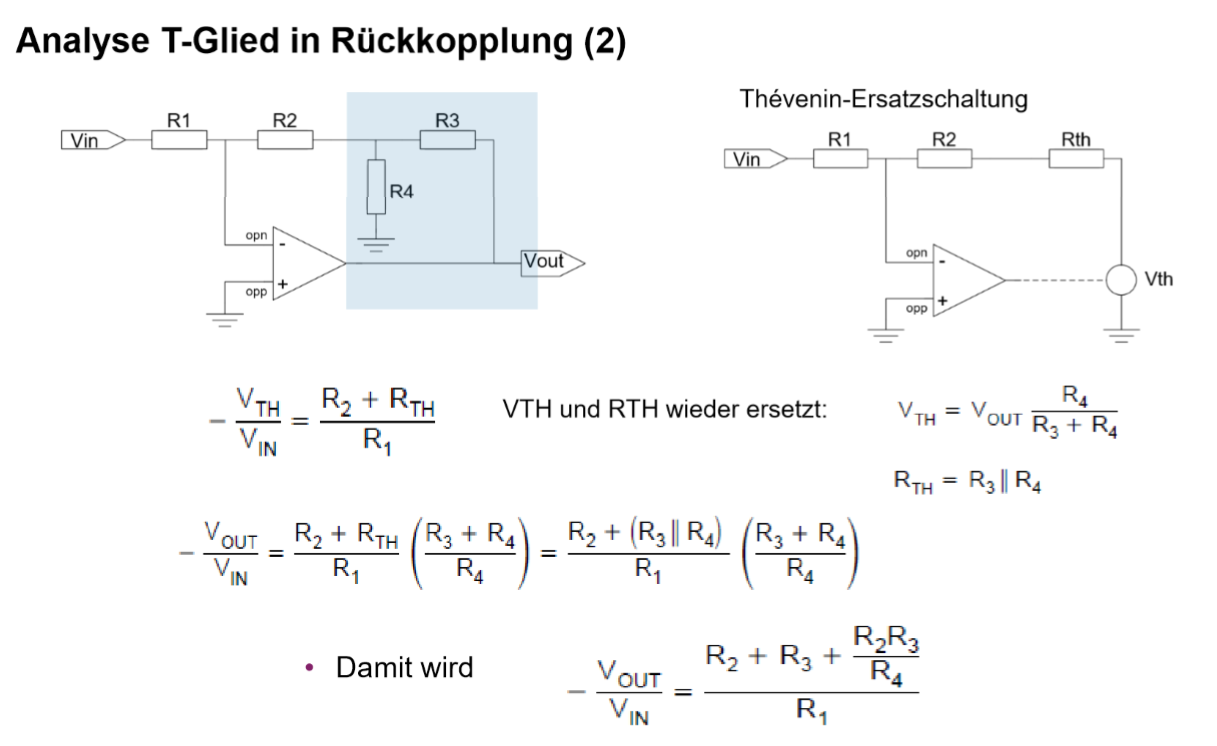
\includegraphics[width=\linewidth,keepaspectratio=true]{./Images/opamp_t-glied}
\end{minipage}%%% to prevent a space
\begin{minipage}{0.30\textwidth}
	\begin{align*}
		-\frac{V_{out}}{V_{in}} &= \frac{R2+R3+\frac{R2R3}{R4}}{R1}
	\end{align*}
\end{minipage}


\subsubsection{Negative Impendanz Konverter}
Parasität reelle Widerstände $-I1$ soll $I_1$ kompensieren. Kein Spannungsabfall über $R_{VIN}$\\
\begin{minipage}{0.20\textwidth}
	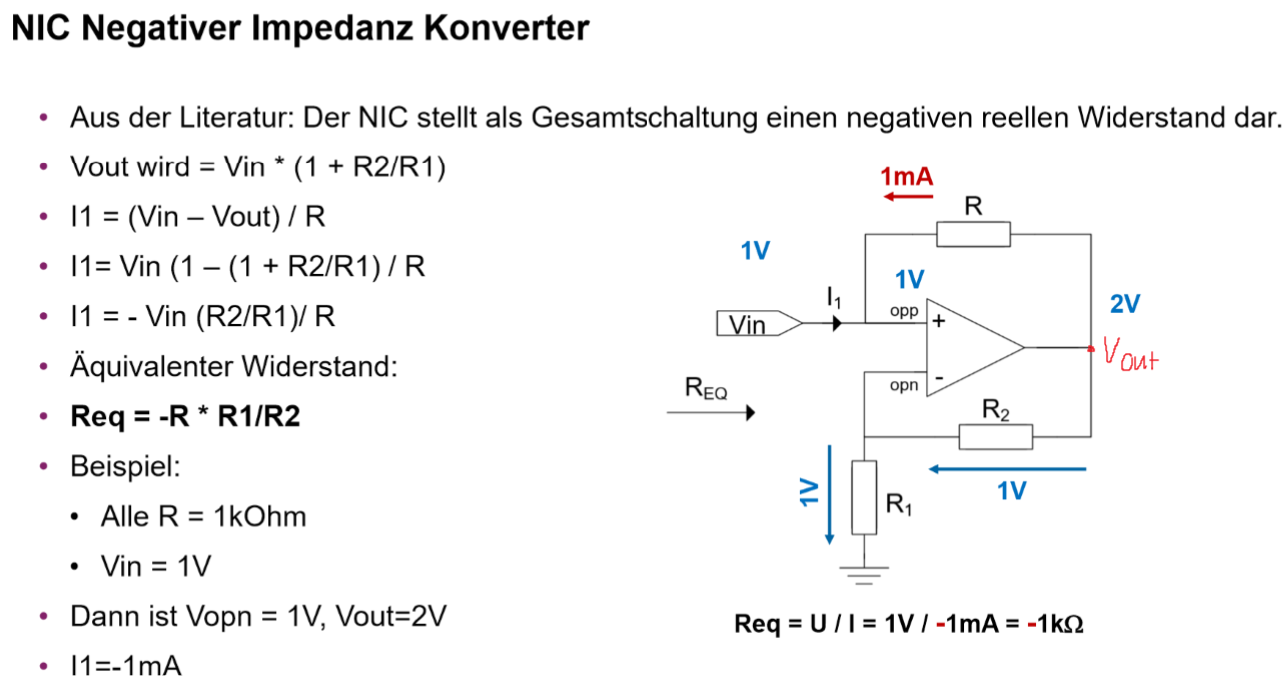
\includegraphics[width=\linewidth,keepaspectratio=true]{./Images/opamp_nic}
\end{minipage}%%% to prevent a space
\begin{minipage}{0.30\textwidth}
	\begin{align*}
		R_{eq} &= -R\cdot \frac{R1}{R2}
	\end{align*}
\end{minipage}


\subsubsection{Komperator}
Bei Komperatoren ist Ausgang entweder $V_{out_{max}}$ oder $V_{out_{min}}$ und die schalten wenn $V_{opp} = V_{opn}$6\\
\begin{minipage}{0.20\textwidth}
	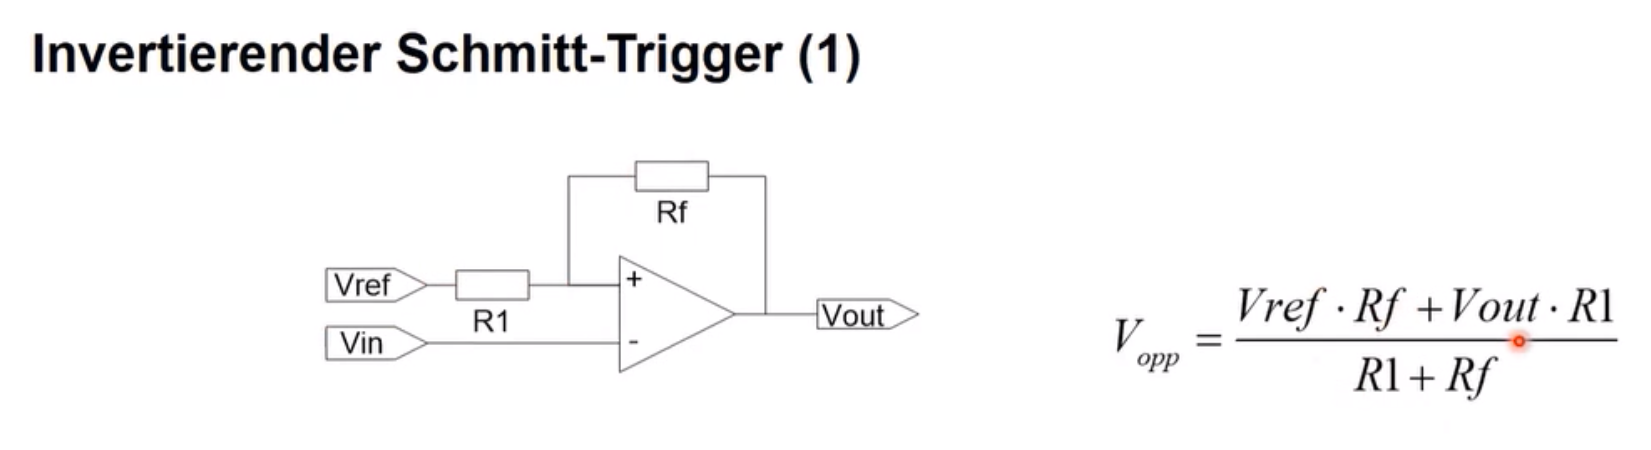
\includegraphics[width=\linewidth,keepaspectratio=true]{./Images/komperator_invertierend}
\end{minipage}%%% to prevent a space
\begin{minipage}{0.30\textwidth}
	\begin{align*}
		V_{opp} &= \frac{V_{ref}\cdot Rf + V_{out_{min/max}}\cdot R1}{R1 + Rf}
	\end{align*}
\end{minipage}

\subsubsection{Integrator}
\begin{minipage}{0.20\textwidth}
	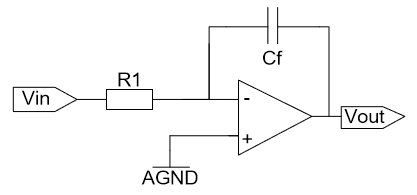
\includegraphics[width=\linewidth,keepaspectratio=true]{./Images/integrator}
\end{minipage}%%% to prevent a space
\begin{minipage}{0.30\textwidth}
	\begin{align*}
		V_{out}(t) &= -\frac{1}{RC}\int_{0}^{t}V_{in}(\tau)d\tau + V_0 \\
		&= -\frac{1}{C}\int_{0}^{t}I_c{in}(\tau)d\tau + V_0
	\end{align*}
\end{minipage}

\subsubsection{Differenzierer}
\begin{minipage}{0.20\textwidth}
	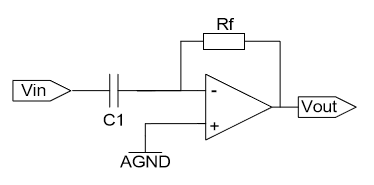
\includegraphics[width=\linewidth,keepaspectratio=true]{./Images/differenzierer}
\end{minipage}%%% to prevent a space
\begin{minipage}{0.30\textwidth}
	\begin{align*}
		V_{out}(t) &= -Rf\cdot C \frac{dV_{in}}{dt}
	\end{align*}
\end{minipage}


\subsection{Nicht idealer Opamp}
Die Eigenschaften eines nicht idealen Operationsverstärker sind:
\begin{enumerate}[nosep]
	\item Offsetspannung	
	\item Offset Strom
	\item Arbeitsbereich
	\item Endliche Verstärkung	
\end{enumerate}

\subsection{Dynamische Eigenschaften}
Die Verstärkung eines Opamp sinkt mit höhere Frequenz. Das \textbf{Gain Bandwidth Product} oder kurz GBP beschreibt dabei die $A(f)$ Verstärkung zu Frequenz Funktion.
\[
A(f) = \frac{A_0}{1 + \frac{A_0}{GBP}\cdot jf}
\]
\begin{center}
	\includegraphics[width=0.4\linewidth]{Images/opamp_dynamische_verstärkung}
\end{center}

Produkt von 3dB-Knickfrequenz (=Bandbreite) und Verstärkung (von pos. Eingang = $\frac{1}{\beta}$) ist konstant

\subsection{Slew-Rate}
Slew-Rate (SW) bezeichnet mögliche Änderungsgeschwindigkeit der Ausgangsspannung
\[
SR = \left|\frac{dV_{out}}{dt}\right|_{max}
\]
